\documentclass{beamer}
\usepackage{xcolor}
\usepackage{mathtools}
\usetheme[titlepagelogo=firenze,% Logo for the first page
		  language=italian,
		  bullet=circle,
		  color=blue,
         ]{TorinoTh}
\usepackage[beamer,customcolors]{hf-tikz}
\definecolor{UniBlue}{RGB}{83,121,170}
\setbeamercolor{block title}{use=structure,fg=white,bg=UniBlue}
\setbeamercolor{block body}{use=structure,fg=black,bg=white}

\newcommand*{\bfrac}[2]{\genfrac{}{}{0pt}{1}{#1}{#2}}

\author{}
\rel{{\normalsize \emph{Visual and Multimedia Recognition}}\\\vspace{0.3cm}Lorenzo Cioni}
\title{\huge Improving WATSS web application with Computer Vision techniques}
\date{}

\begin{document}

\titlepageframe

\begin{tframe}{Introduction}

WATSS, \textbf{Web Annotation Tool for Surveillance Scenarios}, is a web-based annotation tool developed to annotate dataset in surveillance systems.

\vspace{0.3cm}

\textbf{Main goal}: improve WATSS with some \textbf{Computer Vision approaches}, in order to make easy for users to use this tool and make the annotation process more \emph{automatic}

\begin{figure}[h]
\begin{center}
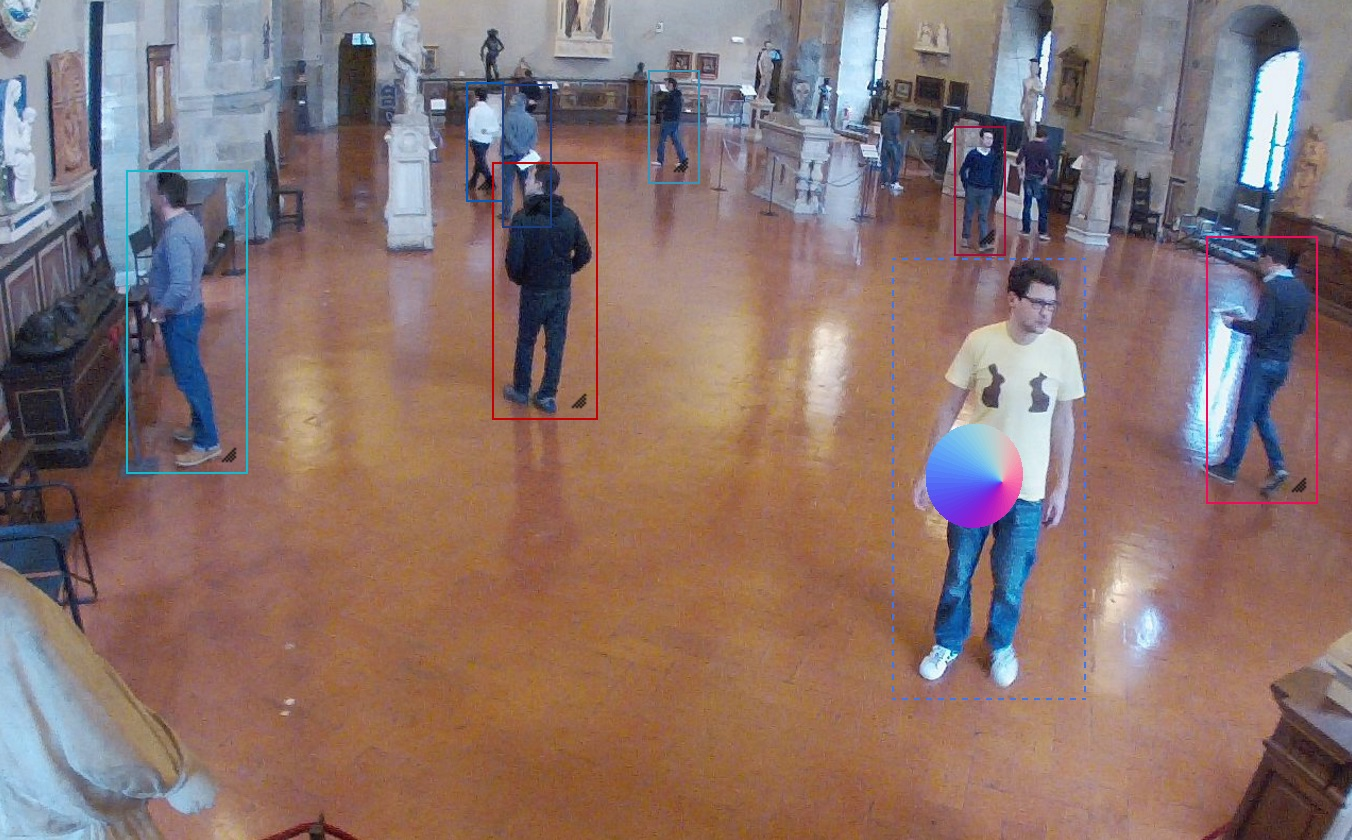
\includegraphics[width=0.4\textwidth]{images/frame.jpg}
\end{center}
\label{fig:mainframe}
\end{figure}

\end{tframe}

\begin{tframe}{Comparative analysis on annotation tools}

\textbf{LabelMe}

\begin{columns}[t]
\begin{column}{0.35\textwidth}
\vspace{0.5cm}
\begin{itemize}
\item Web-based tool, also for mobile applications
\item Annotate scenes with polygonal areas
\item Nested objects and occlusion annotation
\item Zoom in and out of the scene
\end{itemize}
\end{column}
\begin{column}{0.4\textwidth}
\begin{figure}[h]
\centering
\includegraphics[scale=0.15]{images/lire.png}
\end{figure}
\end{column}
\end{columns}



\end{tframe}



\end{document}